\documentclass[10pt,a4paper]{article}
\usepackage[utf8]{inputenc}
\usepackage[english]{babel}
\usepackage{amsmath}
\usepackage{amsfonts}
\usepackage{amssymb}
\usepackage{graphicx}
\usepackage{mathtools}
\usepackage{multirow}
\usepackage{gensymb}
\usepackage{float}
\usepackage[section]{placeins}
\usepackage[left=2cm,right=2cm,top=2cm,bottom=2cm]{geometry}
\author{Elisha B. Are, Jonathan Dushoff, John W. Hargrove}
\title{Estimating the Intrinsic Rate of Natural Increase (IRNI) for tsetse ({\it Glossina} spp) population}
\begin{document}
\maketitle

\section*{Abstract} 
Climate change may have started altering tsetse (vectors of trypanosomiasis) population’s distribution in Africa. Environments that were initially unsuitable for them, may now be getting warm enough to support the flies.  It is therefore important to understand the possibility of both tsetse population extinction, in areas that are now getting too hot for them, as well as, the chances of them surviving in cooler regions that are now getting warmer. The intrinsic rate of natural increase $r$ is a useful metric in determining the suitability of a set of environmental condition for insect population establishment.  The relatively simple life history of the tsetse allows us to solve the Euler-Lotka equation to obtain a closed form expression for $r$. We use daily average temperatures for the Zambezi valley of Zimbabwe (1960 - 2018) to calculate long time average values of $r$. And we created three climate change scenarios for the next 50 years, using daily average temperature data for 2018 as a baseline. Our results show that the growth rate is positive and relatively stable during the cooler seasons, for most of the years of the study period. However, since 2010, tsetse population has been experiencing negative growths more frequently during the hot dry season (October – December).  We found that if daily average temperature continues to increase at the rate of 0.08\degree C per year in the Zambezi valley, tsetse population will go extinct within the next 50 years.   



\section*{Introduction} 

Tsetse ({\it Glossina} spp) are vectors of human and animal trypanosmiasis - a neglected tropical disease - endemic in many sub-Saharan African countries. Sustained control efforts have reduced disease burden in the last 10 years \cite{WorldHealthOrganizationWHO2018}.  However, a recent study showed that climate warming may alter tsetse distribution in Africa: in one hand leading to local extinction of tsetse population in, for instance, the Zambezi valley of Zimbabwe. On the other hand, leading to emergence of tsetse and trypanosomiasis in regions that were initially too cold for the flies \cite{Lord2018}. There is a need for an improved understanding of tsetse population growth as a function of changing temperature.\\ 


The intrinsic rate of natural increase $r$ is an important metric in insect population dynamics as it can be used to determine whether or not a set of environmental condition is suitable for an insect population \cite{Birch1948}. Several attempts have been made to estimate the natural rate of increase for tsetse population . Some of the methods/assumptions used in a number of those works were invalid, yielding results which are not reflecting the true growth rate of tsetse populations in the wild \cite{VanSickle1988a}. Moreover, we could not find any study in the literature that estimated tsetse population growth rates as a function of field temperatures. 
A standard means of estimating the natural rate of increase for populations is the Euler-Lotka (E-L) equation \cite{Birch1948,Zidon2015}, given in discrete form as:

\begin{equation}
\label{equation3}
\sum \lambda^{-x}l_{x}m_{x} = 1.
\end{equation}

where  $l_{x}$ is the probability at birth, that a female individual is alive at age $x$ and $m_{x}$ the expected number of female offspring produced in a unit time by a female aged $x$.  \\ 

The basic reproduction number $R_{o}$ is:
\begin{equation}
\label{equation4}
R_{o}= \sum l_{x}m_{x}. 
\end{equation}

Tsetse have a relatively simple life history; they produce a single larva at regular intervals (+/- 2 days) \cite{Ackley2017}. The mortality rate is higher in newly emerged adult flies than in mature adults, and as the fly grows older, the mortality rate increases slightly \cite{Hargrove2013b}.   The very basic life history of tsetse allows us to obtain a closed form solution of the E-L equation to derive an expression for the intrinsic rate of natural increase for tsetse population. We estimated the rate of increase per-day as a function of daily average temperature for the Zambezi valley from 1960 to 2018, and we calculated long time averages of the  rate of increase. Furthermore, we created three climate warming scenarios (0.04 \degree C, 0.06 \degree C and 0.008 \degree C annual increase), over the next 50 years,  using the daily average temperature data for 2018 as a baseline. We calculated the average annual growth rate for each of the warming scenarios to determine if the annual growth rate will reduce to a negative value within the next 50 years.     


\section*{Materials and Methods}
We sub-divide tsetse life-cycle into three distinct stages, namely, larval/pupal, newly emerged and larvipositing adult stages. Tsetse are a well-studied insect; and so their birth, development, and mortality rates have been measured both  in  the laboratory and  in the field \cite{Rogers2011,Hargrove2004a,Jarry2007,Hargrove2011,Hargrove2019a}. With this knowledge and their relatively simple life-cycle, we present a framework which allows us to solve Euler-Lotka equation analytically for the intrinsic rate of increase for tsetse population. We proceed by making the following simplyfing  assumptions.   
\section*{Model assumptions} 
\begin{itemize} 
	\item  Once the fly attains the age of first ovulation, it retains constant fecundity rate throughout her life.   
	\item We assume that the life-cycle of the fly is divided into three stages, pupa, newly emerged adults and larvipositing adults. 
		\item  $p_o$ is the probability of reaching the larviposition loop from "birth"
	\item   $p_c$ is the probability of reaching the point where offspring are counted, from the point of larviposition.
	\item   $c$ is the time interval between successive "births" (which is assumed to be constant). 
	\item   $p_l$ is the probability of surviving a larviposition loop.
\end{itemize}


\section*{Model} 

Suppose  $l_{x}$ be the probability at birth of, a female, being alive at age $x$, $m_{x}$ the mean number of female offspring produced in a unit time by a female aged $x$.  




\subsection*{Basic reproduction number}

The basic reproduction number $(R_o)$ can be calculated directly from equation (\ref{equation4}): 

$$R_{0 }=\sum l_{x}m_{x},$$
$$x=c,2c,3c,... \implies \frac{x}{c}=y = 1,2,3,...$$ 
where
\begin{equation}
\label{equation6} 
l_{1}=p_op_l, l_{2}= p_op_l^2, l_{3}=p_op_l^3, . . .
\end{equation}
and
\begin{equation}
\label{equation7} 
m_{1}=p_c, m_{2}=p_c, m_{3}=p_c, . . .
\end{equation}
Therefore, from equations (\ref{equation4}),  (\ref{equation6}), and  (\ref{equation7}),

$$R_{0 }=\sum l_{y}m_{y} = p_op_lp_c + p_op_l^2 p_c + p_op_l^3p_c + ...$$

$$=p_op_cp_l (1 + p_l + p_l^2 + p_l^3 + ...),$$
\begin{equation}
\label{equation8} 
=\frac{p_op_cp_l}{(1-p_l)},
\end{equation}
where $0 < p_l < 1$. Notice that $R_o$ does not depend on $c$, moreover, if $p_o$ or $p_c \rightarrow{0}$, then $R_o \rightarrow{0}$. This implies that whenever any of the parameter approaches $0$, the population goes extinct. \\

Equation  (\ref{equation8}) corresponds to the net reproduction number for tsetse population, in the general model presented in \cite{Are2019a}.

\subsection*{The intrinsic rate of natural increase}
We can calculate the intrinsic rate of natural increase $r$ from the  Eular-Lotka equation.  Suppose all parameter descriptions remain as above, we can rewrite equation (\ref{equation3}) by letting $\lambda= e^{cr}$. Equation (\ref{equation3}) then becomes:
\begin{equation}
\label{equation1008} 
\sum (e^{rc})^{-T}l_{T}m_{T}.
\end{equation}
where $ T $ is the integer number of time steps. \\

Using equations  (\ref{equation6}) and  (\ref{equation7}), we can calculate $r$ directly from equation (\ref{equation1008}).

$$\sum (e^{rc})^{-T}l_{T}m_{T} = p_op_lp_c(e^{rc})^{-1} + p_op_l^2p_c(e^{rc})^{-2} + p_op_l^3p_c(e^{rc})^{-3} + ...=1,$$



$$p_op_cp_le^{-rc} (1 + p_le^{-rc} + p_l^2e^{-2rc} + p_l^3e^{-3rc}+ ...) =1,$$

\begin{equation}
\label{equation9} 
\frac{p_op_cp_le^{-rc}}{1-p_le^{-rc}} =1.
\end{equation}
Solving for $r$ in equation (\ref{equation9}) , yields, 

\begin{equation}
\label{equation13} 
r = (\frac{\ln[p_l(p_cp_o+1)]}{c}).
\end{equation}
If  $p_o$ or $p_c \rightarrow{0}$, then  $r \rightarrow{\frac{\ln[p_l]}{c}}$. Since $0 < p_l < 1$, whenever any of the parameters approaches $0$, $r$ becomes negative, which implies  population extinction. Moreover, $r = 0, \implies R_o = 1$.  


\subsection*{Intrinsic growth rate as a function of temperature}

We assume that key parameters are temperature dependent. The relationship between these parameters and temperature are given in detail in \cite{Are2019}. We estimated the rate of increase per-day as a function of daily mean temperature, and we obtained the long-time (annual) average ($\hat{r}$)  of $r$, using: 

\begin{equation}
\label{equation1010} 
\hat{r} = \frac{1}{N} \sum_{t=1}^{N} r_t
\end{equation}

\subsection*{Temperature Data}
For 60 years running, maximum and minimum temperatures are being recorded daily at Rekomitjie, Zimbabwe. Measurement are taken with a mercury thermometer placed in a Stevenson screen.  These readings are used to calculate the daily average temperatures from January 1960 to December 2018. Details about the temperature data are provided elsewhere \cite{Lord2018}.   

\subsection*{Climate change scenarios}

The average daily temperatures have increased by 2\degree C in the month of November, and by 0.9\degree C for the rest of the year, in the past 27 years in the Zambezi valley of Zimbabwe \cite{Lord2018}. Here we project three climate change scenarios.

\begin{itemize}
	\item 	Temperature continues to increase, but the rate of increase is  slow, i.e., the daily average temperature will increase by 0.04\degree C  per-year. 
	\item The rate of increase in the daily average temperatures is 0.06\degree C  per-year  
	\item Temperature increases fast with a rate 0.08\degree C  per-year.    
	This information will be used to generate temperature data for the Zambezi valley, for the next 50 years. 	
\end{itemize} 
 Our goal is to determine if the annual growth rate in the Zambezi valley will attain negative value within the next 50 years.

\section*{Results}

We used the daily average temperature data and equation (\ref{equation13}) to calculate the intrinsic rate of natural increase of tsetse population in the Zambezi Valley of Zimbabwe, from January 1960 to December 2018. We then used equation (\ref{equation1010}) to obtain long time averages for $r$.  We created three climate change scenarios over the next 50 years, using 2018's daily average temperature  as the baseline. We used these temperature projections to calculate the annual average value of the growth rate from 2019 to 2068.  \\

From 1960 to 1986, the annual average growth rate was between 0.00389 at the maximum and 0.00285 at minimum. There were a number of years that the growth rate was really low (for example 1971 and 1976), but the growth rate was also high for other years, making  the average growth rate to be relatively stable over this period (1960 -1986). In 1987, the growth rate hit an all-time low of 0.00287. From 1987 onwards, the average annual growth rate has consistently fall below 0.0038.  From 2010 to 2018, the average growth rate has dropped even further, hitting a new all-time to of 0.0023 in 2016 (Fig \ref{fig:tsetseflowchat0}).      

\begin{figure}[hbt!]
	\centering
	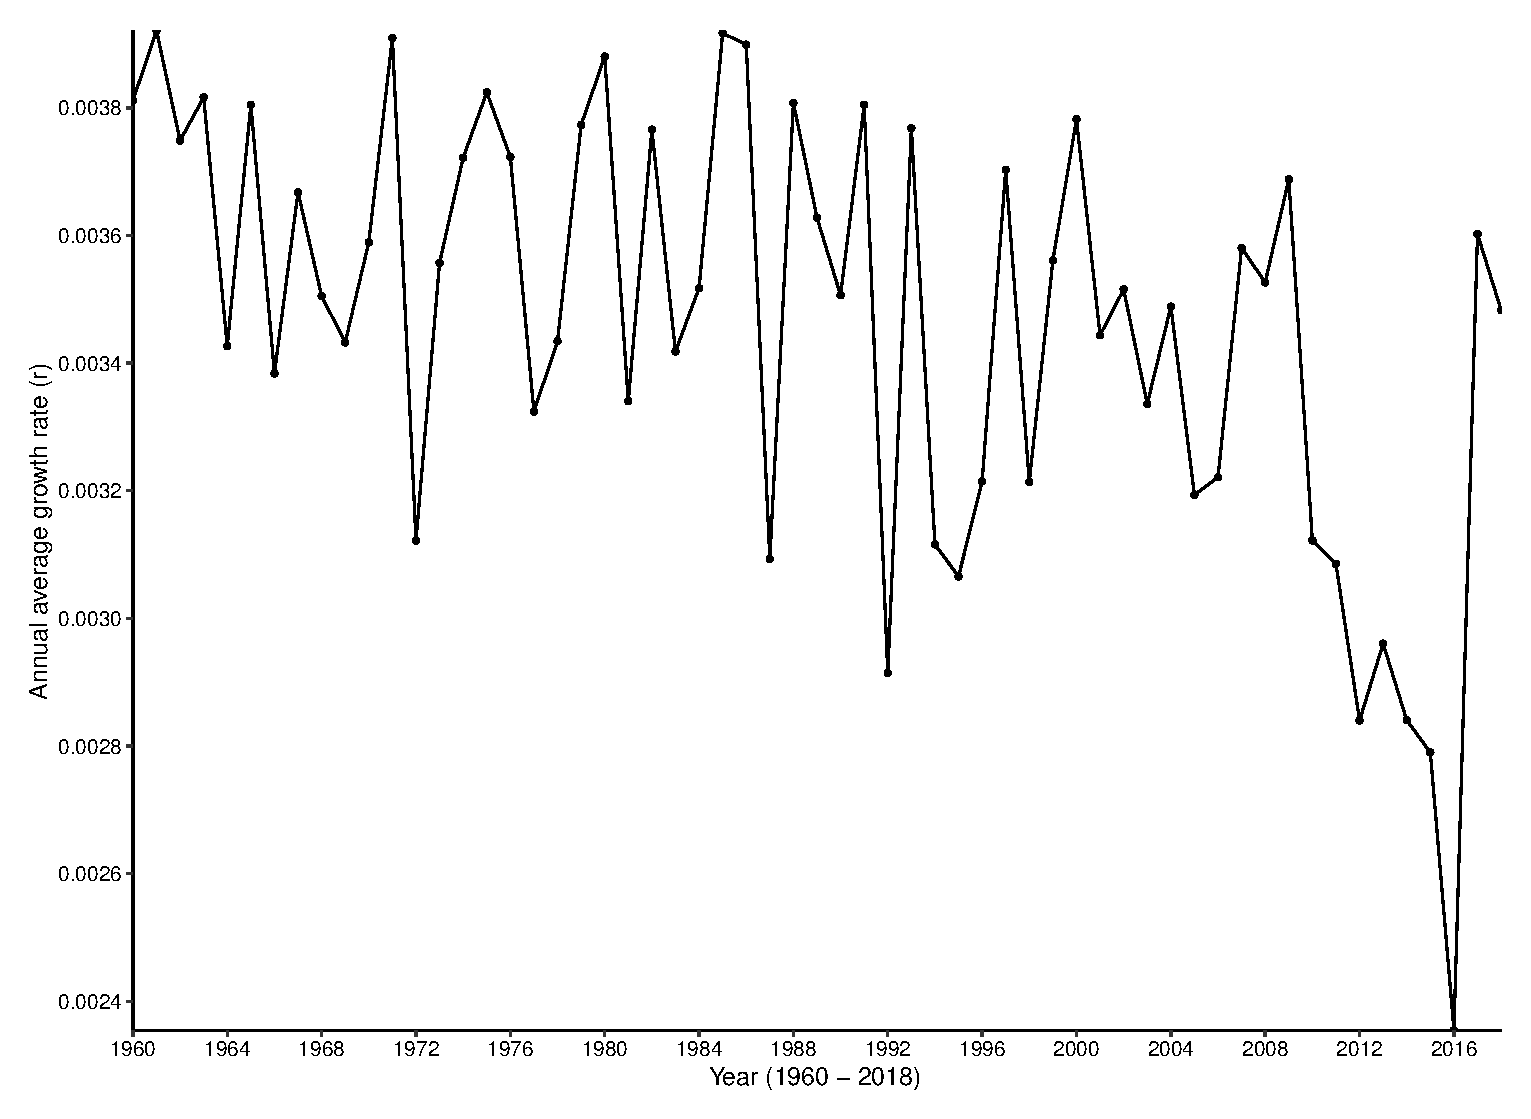
\includegraphics[width=0.6\linewidth]{Check1}
	\caption{Averaged annual growth rate for tsetse population in the Zambezi valley of Zimbabwe: from 1960 to 2018. }
	\label{fig:tsetseflowchat0}
\end{figure}

Temperatures vary seasonally, and higher temperatures are usually recorded during the hot-dry season (October – December). We classified each year from 1960-2018 into three classes as follows: first class consists of months from January to April, the second class includes months from May-August and the last class consists of months between September and December, inclusive. For each of these classes we obtained the average growth for each month, separately, throughout the study period. This is to allow us assess the differential values of the average growth rate during the hot dry seasons and the much cooler seasons of the year. The average growth rate did not change much for months between January and April save for 1996 and 2016, where the average growth rate dropped markedly in January and February. In general, the average growth rate was about 0.0045 on the average, from January to April, with more fluctuations recorded from 1992 onwards (Fig \ref{fig:tsetseflowchat2}A).\\     





\begin{figure}[h]
	\centering
%	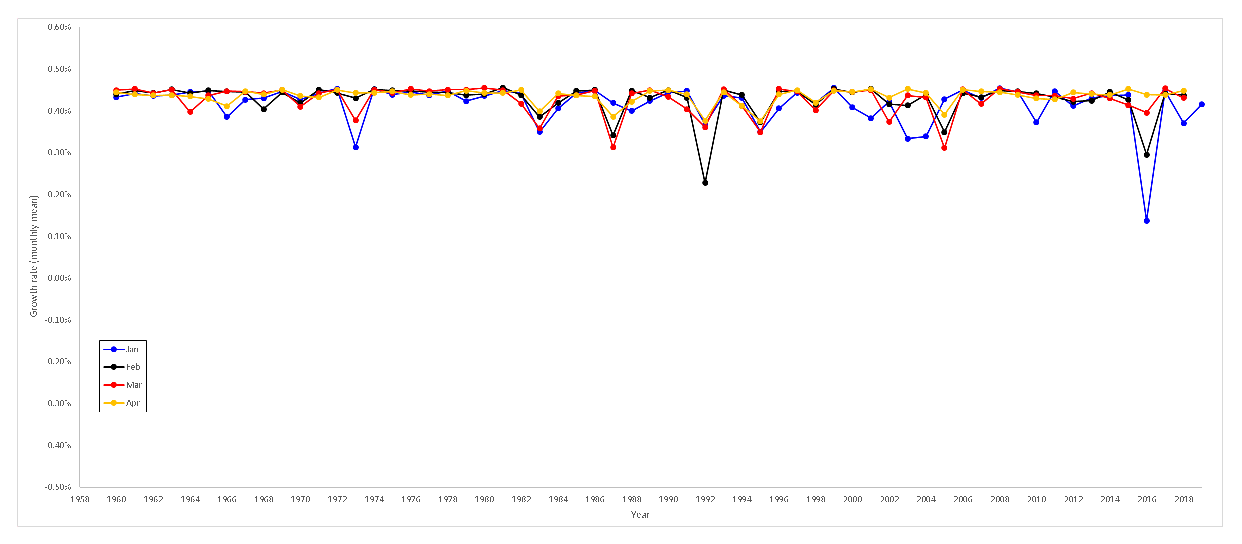
\includegraphics[width=0.9\linewidth]{Jan-April}
%	\caption{Average growth rate for January, February, March and April, from 1960 to 2018.}
	\label{fig:tsetseflowchat1}
\end{figure}

For months starting from May to August (the cooler time of the year),  the average growth rate did not vary much during these months. The growth rate attains it highest value, during this period, the growth rate is about 0.004. The average growth rate is less during  June and July compared to May and August, for every year, during the study period  (Fig \ref{fig:tsetseflowchat2}B).  



\begin{figure}[h]
	\centering
	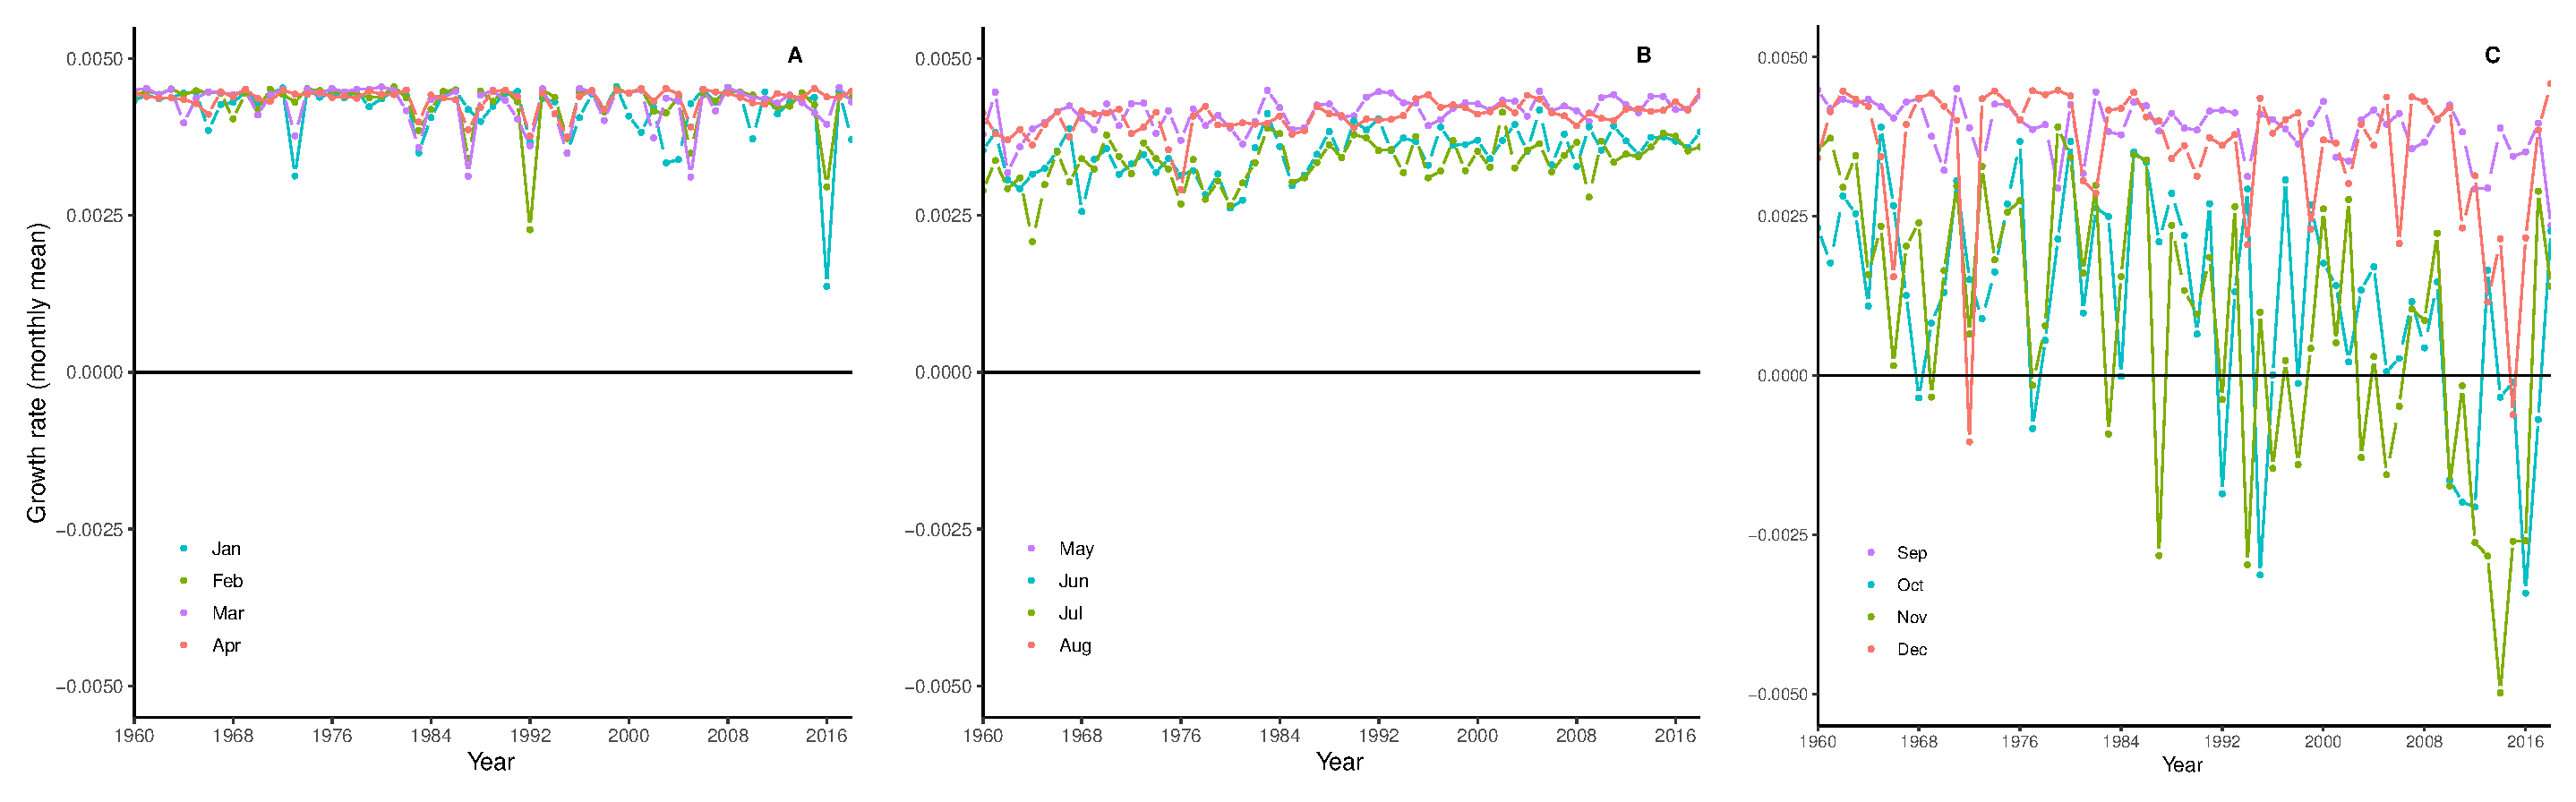
\includegraphics[width=1.05\linewidth]{MonthlyGrowthRateDec12}
	\caption{ {\bf The average growth rate for different seasons from 1960 to 2018} (A). Average growth rate for January, February, March and April (B). Average growth rate for May, June, July and August (C). Average growth rate for September, October, November and December. The horizontal lines shows the limit of positive growth; below those lines the population size decreases}
	\label{fig:tsetseflowchat2}
\end{figure}

\newpage
There is a major variation in the average growth rate during the last four months of the year. From 1987 to 2018, the average growth rate has been negative for most of the years, during October and November. On a closer inspection, we found only a modest variation in the values of the average growth rate for September, from 1960 to 2010, save for the sharp drop it experienced in 1972. From 2010 to 2018, there have been notable variations in the value of the growth rate during the last for months of the year. During this period, the growth rate usually hits its lowest value during November or October.  In 2014, the growth rate dipped below -0.005 - it lowest monthly average ever (Fig \ref{fig:tsetseflowchat2}C). 



\begin{figure}[h]
	\centering
	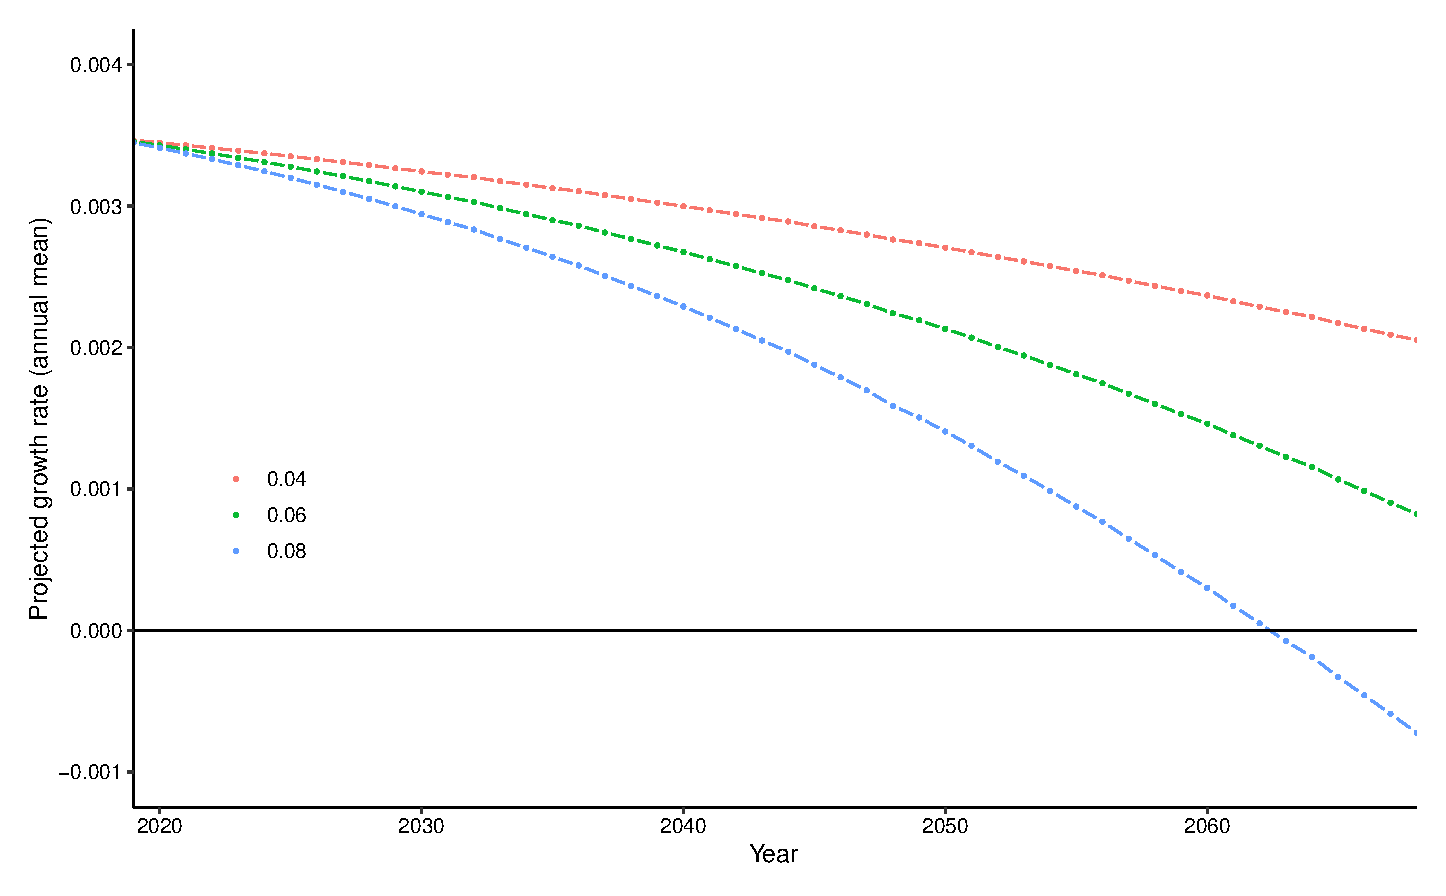
\includegraphics[width=0.8\linewidth]{Projected_growthRateDec12}
	\caption{{\bf The annual average growth rate for the three projected climate change scenarios (0.04, 0.06, 0.08 \degree C per-year), from 2019  to 2068}. The horizontal line, through the vertical axis, shows the point where the average growth rate attains negative values: indicating population extinction.}
	\label{fig:tsetseflowchat4}
\end{figure}

When the warming rate is slow (at 0.04 \degree C per-year), the average growth rate continues to decline as temperature increases, but it did not reach a negative value within the next 50 years. For the scenario where the warming rate is  0.06 \degree C per-year, the $\hat{r}$ drops below 0.001 but did not reach a negative value. Moreover, when the warming rate is increased to  0.08 \degree C per-year, $\hat{r}$ declines steadily until it reaches a negative value in 2063. A negative $\hat{r}$ value indicates population extinction. 
 



\section*{Discussion}

A study showed that increasingly high temperature in the Zambezi valley is responsible for the observed collapse in tsetse population in that region. And the study proposed that if average temperatures continue to increase, there might be local extinction of tsetse population in the Zambezi valley \cite{Lord2018}.  The current study showed how tsetse growth rate has changed over the past 60 years and predicted the time to extinction for tsetse population in the Zambezi valley given different climate change scenarios.  We solved the E-L equation analytically, and we obtained a closed form expression for the intrinsic growth rate $r$ for tsetse populations. We used the daily average temperature for the Zambezi valley, from January 1960 to December 2018, to calculate the long-time average values of $r$. Using the temperature readings for 2018, we projected three climate change scenarios, by generating daily average temperatures for the Zambezi valley over the next 50 years, following three climate warming rates. We used the projected temperatures to calculate the long-time averages of the growth rate.    \\

Our results show that tsetse population growth rate, for the Zambezi valley, has fluctuated year-in-year-out,  over the past 60 years. From the 1990s when the average temperatures have increased markedly, the annual average growth rate has continued to reduce.  Our results agree with several studies \cite{Pagabeleguem2016f,Ackley2017}, both empirical and theoretical, that have shown that high temperatures are devastating for tsetse populations, and that increasingly high temperatures can drive tsetse populations to extinction\cite{Lord2018,Are2019}. Our results offer insight into how very high temperatures during the hot-dry season is responsible for the decline in tsetse population in the Zambezi valley. During the hot-dry seasons, the very high mortality rates in both pupal and newly emerged adult stages are sufficient to cause negative growth rates, during these months. The proceeding seasons will require highly favourable conditions for the population to rebound before the next hot dry season.  As global warming continues to increase the average temperatures in the Zambezi valley all year round, tsetse population will not be able to recover fully from the disastrous impact of the hot-dry season before the next hot-dry season set in, since the initially favourable seasons are no longer as favourable. This may explain the decline in tsetse population, in the Zambezi valley, over the past 10 - 20 years. It is worthy of note that although the annual average values of $r$ may be positive, it does not necessarily mean that the population is growing, as our estimate is reflecting only the best case scenarios given the environmental condition, in this case temperature. Our result can be seen as an instantaneous  maximum growth rate attainable for tsetse population in the Zambezi valley \\

We have shown that tsetse populations have very low growth rates. For instance, from the 1960s to 1980s where the environmental temperatures were relatively favourable throughout the year, the annual average growth rate was always below 0.004 per-year. This is consistent with the vary low tsetse birth rates \cite{Hargrove2004a,HARGROVE1988}. Other studies have also estimated very low population growth rates for tsetse populations \cite{VanSickle1988,Hargrove2004a}. We have assumed that no additional mortality is imposed on the study population either by control efforts [ref] or human activities i.e., bush clearing. If any of these assumption is not true, then tsetse growth rate will be less than what we present here. Our result may therefore be a best case scenario for tsetse population which are experiencing the temperatures recorded in the Zambezi valley during these periods \\


We acknowledge that the E-L equation was premised on the assumption that the population attains a stable age distribution, and where the environment is not limited by resources or space. Some may then argue that tsetse population cannot attain stable age distribution in the field \cite{VanSickle1988}. We argue that this will does not invalidate our results as a first stab at estimating the tsetse growth rate in the field, and the insight it offers into tsetse population extinction in the Zambezi valley,  because of the following reasons. Amarasekare et al \cite{Amarasekare2013} provided strong evidence that populations can still attain stationary age distributions as long as the fluctuation in environmental temperature is within a thresh hold that will allow reproduction and development processes to continue. We have shown that for most months of the year, in the Zambezi valley, apart from the hot dry seasons, temperature variations have been minimal. The instability in the age distribution is often introduced during the hot-dry seasons \cite{Hargrove2013b} of the very hot years. Our estimate may not be accurate to very high degrees but it does provide a very insightful first step towards a more accurate estimates of tsetse population growth rate under varying temperatures.  \\

The current study did not consider density dependent effects. It is worth stating though that density dependence effect are very important in the study of insect populations, especially for tsetse population which can be seriously affected by density dependent effects \cite{Rogers1975}. However, the E-L equation has been shown to yield  comparable estimates of $r$ to other methods that incorporated density dependent effects. A study \cite{Cortes2016} did an extensive comparison of five different methods for estimating $r$ for a fish population and they reported that the density independent assumption on which E-L equation is derived does not limit it validity of the $r$ estimates derived from it.    \\



A study \cite{Amarasekare2013} compared the average growth rate calculated from the E-L equation to the one obtained from a stage-structured compartmental model. They reported that the growth rates obtained from the two methods compared well, deviating only when the juvenile developmental period is long (several months) and/or when projections involve long time-scale ($>$ 50 years).  When the two estimates differs, $r$ derived from the E-L equation overestimates the true growth rates, and by implication, it overestimates population persistence. They suggested that the accuracy of $r$, from the L-E method, declines if it is used to predict insect population extinction beyond a 50-year period.  The current study took these cautions into account.  Moreover, tsetse developmental period can vary between 20 - 60 days depending on temperature, and it therefore can be categorized as having a relatively  short developmental period.   In any case, the shortcoming of our method will be that tsetse populations may more likely to go extinct earlier than in 2063 that was predicted by our results. 


\section*{Conclusions}
The framework presented here is simple and relatively straightforward. We recognize that some of the shortcomings of our formulation may limit the accuracy of our estimates.  However, among other things, since we got a closed form expression for $r$, it will serve as a metric to easily compare future findings with. Moreover,  it is clear that this crude estimate provides a strong evidence that climate change may drive several tsetse populations to extinction within the next 50 years (with a medium warming rate of 0.08\degree C per-year), especially in temperate regions with similar temperature profile as  the Zambezi valley. If our results are true for other insects with similar reproduction/development processes to tsetse, then several insects, of agricultural and/or economic importance, may be at risk of extinction in the Zambezi valley in particular, and Zimbabwe ( or other part of Africa with similar temperature regimes as the Zimbabwe),  in general. \\

We are currently constructing an individual based model which will allow us to factor in several environmental variables at the same time, to estimate the actual growth rate of tsetse population in the wild. This will be used to compare the current results. 

\bibliographystyle{ieeetr}
\nocite{*}
\bibliography{Growthrate}
\end{document}





%%%%%%%%%%%%%%%%%%%%%%%%%%%%%%%%%%%%%%%%%%%%%%%%%%%%%%%%%End of article%%%%%%%%%%%%%%%%%%%%%%%%%%%%%%%%%%%%%%%%%%%%%%%























\begin{figure}[hbt!]
	\centering
	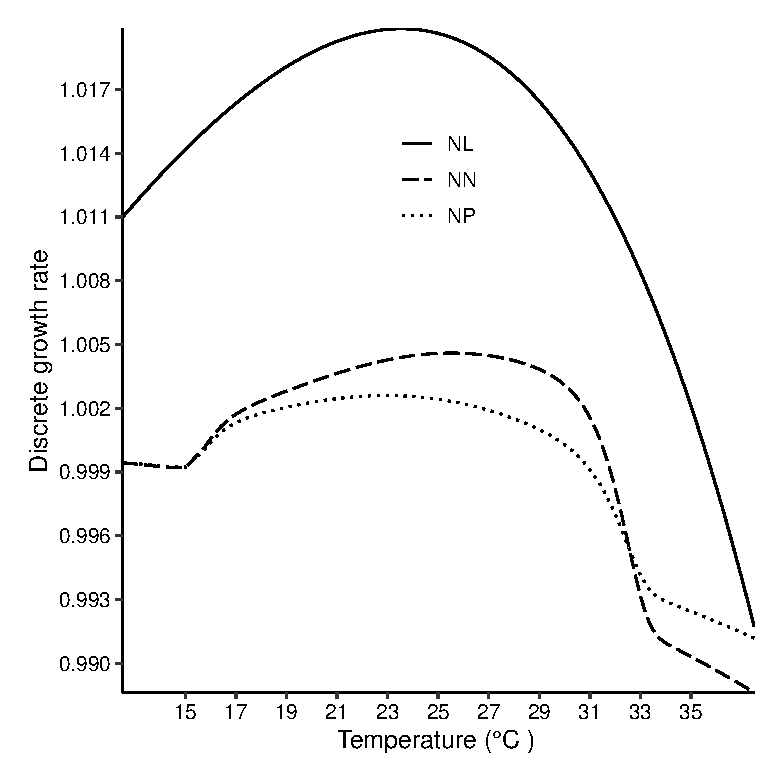
\includegraphics[width=0.7\linewidth]{NLNP}
	\caption{Discrete growth rate as a function of temperature}
	\label{fig:tsetseflowchat3}
\end{figure}





\begin{figure}[hbt!]
	\centering
	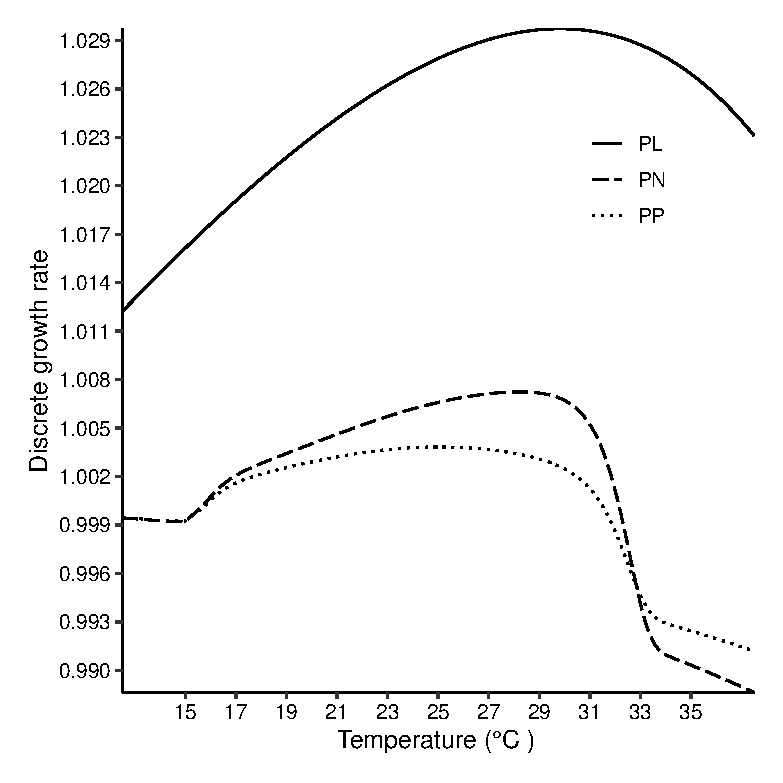
\includegraphics[width=0.7\linewidth]{PLPP}
	\caption{Discrete growth rate as a function of temperature}
	\label{fig:tsetseflowchat3}
\end{figure}

\newpage 

\section*{Possible way forward?} 

\begin{itemize}  
	\item  We can estimate the growth rate $\lambda$ for a year (with annual average temperature). 
	
	\item We can then use the temperature data for the Zambezi valley of Zimbabwe to estimate $\lambda$ for tsetse population over the past years. If our results are meaningful, we can proceed by estimating  $\lambda$ to assess tsetse population growth rate for different temperature projections. We can ask questions like, if the annual average   temperature continues to increase at the present rate, at what year will $\lambda < 1$ Or could the values of $\lambda$ explain the decline in tsetse population in the last few years, in the Zambezi valley of Zimbabwe? 
\end{itemize}












\newpage
\subsubsection*{Remark I} 

We note here that the "count point" may differ from the "birth point" (i.e. the birth point is the stage at which the parent is counted, while the "count point" is the stage at which the offspring are counted). Below we present a  table of all possible scenarios. 


\begin{table}[h!]
	\centering
	\begin{tabular}{ |c|c|c|c| } 
		\hline
		& $L$ & $N$ & $P$ \\
		\hline
		$L$ & $LL$ & $LN$ & $LP$\\ 
		\hline
		$N$& $NL$ & $NN$ & $NP$\\ 
		\hline
		$P$& $PL$ & $PN$ & $PP$ \\ 
		\hline
	\end{tabular}
	\label{table:1}
	\caption{Table of all possible scenerios}
\end{table}

The first colunm lists the stage at which the parent is counted and the first row presents the stage at which the offspring are counted. The diagonal entries represent suitautions where the "count point" and "birth point" are assumed to be the same (e.g for LL, parent starts as a female larva, and offspring are also counted at larval stage). We will like to state here that Table 1 can easily be extended for insects with more than three distinct life stages.




\subsection*{Special cases of the general model}

Birth can be defined defferently in different contexts.  In what follows, we present different possible counting scenarios, to capture differing definitions of 'birth' and 'count' points. \\ Suppose:\\
\begin{itemize}
	\item $p_{de}$ is the probability that a deposited larva emerges as a young adult
	\item $p_{eo}$ is the probability that a newly emerged adult survives upto the first ovulation
	\item  $\beta$ is the probability that a deposited larva is female.
\end{itemize}




\subsubsection*{Case 1- LL}

Suppose the parent was at the larval stage when counted and the offspring are also counted as alrvae. We will have:

$$\hat{p_o}= p_{de}p_{eo},$$ and 

$$\hat{p_c}= \beta,$$ Substituting the above into equations (\ref{equation8}) and (\ref{equation10}) yields:

\begin{equation}
\label{equation88} 
R_o =\frac{\beta p_{de}p_{eo}p_l}{(1-p_l)}.
\end{equation} and 

\begin{equation}
\label{equation101} 
\lambda =(p_l(\beta p_{de}p_{eo}+1))^\frac{1}{c_1},
\end{equation}
where $c = c_1$ (the time interval between each larviposition) 

\subsubsection*{Case 2- LN}

Suppose the parent is counted as a larva, but the offspring are counted when the emerged as young adults. Then 

$$\hat{p_o}= p_{de}p_{eo},$$ and 

$$\hat{p_c}= \beta p_{de},$$
Inserting these into  equations (\ref{equation8}) and (\ref{equation10}), gives

\begin{equation}
\label{equation882} 
R_o =\frac{\beta p^2_{de}p_{eo}p_l}{(1-p_l)}.
\end{equation} 

and

\begin{equation}
\label{equation102} 
\lambda =(p_l(\beta p^2_{de}p_{eo}+1))^\frac{1}{c_1 + c_2},
\end{equation}

where $c = c_1 + c_2$ ( $c_2$ is the time interval between larviposition and emergence as young adult)   


\subsubsection*{Case 3- LP}

Suppose the parent is counted as a larva, but the offspring are counted when they are in the ovulation cycle. Then we have the following:

$$\hat{p_o}= p_{de}p_{eo},$$ and 

$$\hat{p_c}= \beta p_{de}p_{eo},$$
Inserting these into  equations (\ref{equation8}) and (\ref{equation10}), gives

\begin{equation}
\label{equation883} 
R_o =\frac{\beta p^2_{de}p^2_{eo}p_l}{(1-p_l)}.
\end{equation} and

\begin{equation}
\label{equation103} 
\lambda =(p_l(\beta p^2_{de}p^2_{eo}+1))^\frac{1}{c_1 + c_2 + c_3},
\end{equation} 
where $c = c_1 + c_2 + c_3$ ( $c_3$ is the time interval between emergence as young adult and the unset of first ovulation cycle) 

\subsubsection*{Case 4- NL}

Suppose the parent is counted as a newly emerged adult, but the offspring are counted at the larval stage. Then

$$\hat{p_o}= p_{eo},$$ and 

$$\hat{p_c}= \beta,$$
Inserting these into  equations (\ref{equation8}) and (\ref{equation10}), gives

\begin{equation}
\label{equation88} 
R_o =\frac{\beta p_{eo}p_l}{(1-p_l)}.
\end{equation} and

\begin{equation}
\label{equation102} 
\lambda =(p_l(\beta p_{eo}+1))^\frac{1}{c_1},
\end{equation}
where $c = c_1$ (the time interval between each larviposition) 



\subsubsection*{Case 5-NN}

Suppose both the parent and and the offspring are counted at the point of emergence, then:

$$\hat{p_o}= p_{eo} $$ and 

$$\hat{p_c}= \beta p_{de},$$ putting the above into equations (\ref{equation8}) and (\ref{equation10}), we obtain;

\begin{equation}
\label{equation8884} 
R_o =\frac{\beta p_{de}p_{eo}p_l}{(1-p_l)}.
\end{equation} and 


\begin{equation}
\label{equation104} 
\lambda =(p_l(\beta p_{de}p_{eo}+1))^\frac{1}{c_1 + c_2},
\end{equation}
where $c = c_1 + c_2$ ( $c_2$ is the time interval between larviposition and emergence as young adult)  

\subsubsection*{Case 6- NP}

Suppose the parent is counted as a larva, but the offspring are counted when they are in the larviposition cycle. Then we have the following:

$$\hat{p_o}= p_{eo},$$ and 

$$\hat{p_c}= \beta p_{de}p_{eo},$$
Inserting these into  equations (\ref{equation8}) and (\ref{equation10}), gives

\begin{equation}
\label{equation885} 
R_o =\frac{\beta p_{de}p^2_{eo}p_l}{(1-p_l)}.
\end{equation} and

\begin{equation}
\label{equation105} 
\lambda =(p_l(\beta p_{de}p^2_{eo}+1))^\frac{1}{c_1 + c_2 + c_3},
\end{equation} 
where $c = c_1 + c_2 + c_3$ ( $c_3$ is the time interval between emergence as young adult and the unset of first ovulation cycle). 





\subsubsection*{Case 7- PL}

Suppose the parent is counted only when they are in the first larviposition cycle, but the offspring are counted at the larval stage. Then

$$\hat{p_o}= 1,$$ and 

$$\hat{p_c}= \beta,$$
Inserting these into  equations (\ref{equation8}) and (\ref{equation10}), gives

\begin{equation}
\label{equation886} 
R_o =\frac{\beta p_l}{(1-p_l)}.
\end{equation} and

\begin{equation}
\label{equation106} 
\lambda =(p_l(\beta + 1))^\frac{1}{c_1},
\end{equation}
where $c = c_1$ (the time interval between each larviposition) 




\subsubsection*{Case 8- PN}

Suppose the parent is counted only when they are in the first larviposition cycle, and the offspring are counted at the point of emergence as  adults. We have

$$\hat{p_o}= 1,$$ and 

$$\hat{p_c}= \beta p_{de},$$
Substituting these in  equations (\ref{equation8}) and (\ref{equation10}), gives

\begin{equation}
\label{equation886} 
R_o =\frac{\beta p_{de}p_l}{(1-p_l)}.
\end{equation} and

\begin{equation}
\label{equation106} 
\lambda =(p_l(\beta p_{de} + 1))^\frac{1}{c_1 + c_2},
\end{equation}
where $c = c_1 + c_2$ ( $c_2$ is the time interval between larviposition and emergence as young adult)

\subsubsection*{Case 9-PP}

Here, the parent is counted only when they are in the first larviposition cycle, and the offspring are counted only when they are also in the larviposition loop.

$$\hat{p_o}= 1,$$ and 

$$\hat{p_c}= \beta p_{de}p_{eo},$$ then 

\begin{equation}
\label{equation8888} 
R_o =\frac{\beta p_{de}p_{eo}p_l}{(1-p_l)}. 
\end{equation} and

\begin{equation}
\label{equation105} 
\lambda =(p_l(\ \beta p_{de}p_{eo}+1))^\frac{1}{c_1 + c_2 + c_3},
\end{equation} 
where $c = c_1 + c_2 + c_3$ ( $c_3$ is the time interval between emergence as young adult and the unset of first ovulation cycle). 








\subsubsection*{Remark II}

It is clear from equations (\ref{equation88})-(\ref{equation8888}), that the basic reproduction number is the same for all diagonal entries of Table 1. 




\subsection*{Example 1}

Suppose we are counting ovulating adults (already in the ovulating cycle) in the population, it imples that  $\hat{p_o} = 1$ and $p_{de} = \phi^\sigma$ $p_{eo} =\Omega^\nu$. Let $p_{l} = \chi^\tau$. Assuming there are sufficient males to inseminate all newly emerged females in the population, and the following parameter desciption and values. 

\begin{itemize}
	\item $\beta$: probability that a deposited larva is female = 0.5
	\item $\phi$:  pupa daily survival probability = 0.99
	\item $\sigma$: pupal duration = 27 days 
	\item $\chi$:  daily survival probability for ovulating adult = 0.99
	\item $\Omega$:  daily survival probability for newly emmerged adult = 0.98
	\item $\tau$:  Inter-larval period = 9 days
	\item $\nu$:   time  from adult emmergence to first ovulation = 8 days 
	\item $c$:   time between births = $\sigma + \nu + \tau $
\end{itemize}
The intrinsic rate of natural increase, per day; 


$$r = \frac{\ln[\chi^\tau(\beta \Omega^\nu\phi^\sigma + 1 )]}{\sigma + \nu + \tau},$$ $\implies$ $r = 0.00434$ per day. 












































\item Birch, 1948 L. The intrinsic rate of increase of an insect population. Journal of Animal Ecology 17:15–26.
\item Ryan, L. (1981). Glossina (Diptera: Glossinidae) population growth rates.—Bull. ent. Res. 71, 519–531.
\item Saunders, D. S. (1967). Survival and reproduction in a natural population of the tsetse fly, Glossina palpalis palpalis (Robineau-Desvoidy).—Proc. R. ent. Soc. Lond. (A) 42, 129–137
\item Taylor, P. (1979). The construction of a life-table for Glossina morsitans morsitans Westwood (Diptera: Glossinidae) from seasonal age-measurements of a wild population.—Bull. ent. Res. 69, 553–560.
\item Van Sickle, J. (1988). Invalid estimates of rate of population increase from Glossina (Diptera: Glossinidae) age distributions. Bulletin of Entomological Research, 78(1), 155-161. doi:10.1017/S0007485300016175




\begin{center}
	\begin{tabular}{|c|c|c|c|c|}	
		\hline 
		\rule[-1ex]{0pt}{2.5ex}	$x$& $l_x$& $m_x$ & $l_x m_x$ & $e^{-rx}$ \\ 
		\hline
		\rule[-1ex]{0pt}{2.5ex}	1& $\hat{p_o}p_l$ & $\hat{p_c}$ &$\hat{p_o}p_l\hat{p_c}$  &  $e^{-r}$ \\ 
		
		\rule[-1ex]{0pt}{2.5ex}	2& $\hat{p_o}p_l^2$ & $\hat{p_c}$ &$\hat{p_o}p_l^2\hat{p_c}$  &  $e^{-2r}$ \\ 
		
		\rule[-1ex]{0pt}{2.5ex} 3& $\hat{p_o}p_l^3$ & $\hat{p_c}$ &$\hat{p_o}p_l^3\hat{p_c}$  &  $e^{-3r}$ \\ 
		
		\rule[-1ex]{0pt}{2.5ex}	.& . & .&.&  .\\ 
		
		\rule[-1ex]{0pt}{2.5ex}		.& . & .&.&  .\\ 
		
		\rule[-1ex]{0pt}{2.5ex}		.& . & .&.&  .\\ 
		\hline	
	\end{tabular} 
\end{center}

Assuming that the population grows exponentially with nonoverlapping generations, then

\begin{equation}
\label{equation1}
T= \frac{\ln R_{o}}{r},
\end{equation}

where $T$ is the mean length of a generation and $R_o$, the net reproduction rate.  


This method seems to be popular before Van Sickle (1988) pointed out a major shortcoming in the previous studies. Van Sickle warned that, equating survivorship for each age class to  the female in that class divided by number of flies in the youngest age class, and following the procedure proposed in those studies, is valid only  if $r=0$, therefore yielding values of $r$ that are always close to $0$. Van Sickle concluded that although the previous estimates of $r$, proposed by these studies reflect the low growth rate of tsetse ({\it Glossina}) population, it however failed to reflect the true growth rate.





The finite rate of increase $\lambda$ is  the natural antilog of the intrisic rate of increase $r$. 
That is: 
\begin{equation}
\label{equation11} 
\lambda=e^{r}=p_l(\hat{p_c}\hat{p_o}+1)
\end{equation}


Equation (\ref{equation11}) can be written in terms of $R_o$ as:

\begin{equation}
\label{equation12} 
\lambda = R_o + p_l(1-R_o),
\end{equation}

Where $\lambda = e^{r\tau}$,  $\tau$ is the inter-larval period. 



This appears to be a reasonable estimate of $\lambda$, given parameter values above. Moreover, the value of $r$ is very close to those obatined for field populations in earlier studies. 